
%  article.tex (Version 3.3, released 19 January 2008)
%  Article to demonstrate format for SPIE Proceedings
%  Special instructions are included in this file after the
%  symbol %>>>>
%  Numerous commands are commented out, but included to show how
%  to effect various options, e.g., to print page numbers, etc.
%  This LaTeX source file is composed for LaTeX2e.

%  The following commands have been added in the SPIE class 
%  file (spie.cls) and will not be understood in other classes:
%  \supit{}, \authorinfo{}, \skiplinehalf, \keywords{}
%  The bibliography style file is called spiebib.bst, 
%  which replaces the standard style unstr.bst.  

\documentclass[a4paper]{spie}  %>>> use for US letter paper
%%\documentclass[a4paper]{spie}  %>>> use this instead for A4 paper
%%\documentclass[nocompress]{spie}  %>>> to avoid compression of citations
%% \addtolength{\voffset}{9mm}   %>>> moves text field down
%% \renewcommand{\baselinestretch}{1.65}   %>>> 1.65 for double spacing, 1.25 for 1.5 spacing 
%  The following command loads a graphics package to include images 
%  in the document. It may be necessary to specify a DVI driver option,
%  e.g., [dvips], but that may be inappropriate for some LaTeX 
%  installations. 
\usepackage[]{graphicx}
\usepackage{hyperref}
\usepackage{listings}
\hypersetup{
    colorlinks,
    linkcolor={black!50!black},
    citecolor={blue!50!black},
    urlcolor={blue!80!black}
}
\usepackage{pdfpages}
\usepackage{parcolumns}

\usepackage[utf8]{inputenc} 
\usepackage[english]{babel}

\usepackage{color}
\definecolor{lightgray}{rgb}{.9,.9,.9}
\definecolor{darkgray}{rgb}{.4,.4,.4}
\definecolor{purple}{rgb}{0.65, 0.12, 0.82}


\usepackage{array}
\newcolumntype{L}[1]{>{\raggedright\let\newline\\\arraybackslash\hspace{0pt}}m{#1}}
\newcolumntype{C}[1]{>{\centering\let\newline\\\arraybackslash\hspace{0pt}}m{#1}}
\newcolumntype{R}[1]{>{\raggedleft\let\newline\\\arraybackslash\hspace{0pt}}m{#1}}

\usepackage{xcolor,colortbl}
\usepackage{color}
\usepackage{babelbib}


\title{Robot Applications} 

\author{Lars Engel, Vikash, Ahsan Yousuf
\\\textit{\\Faculty of Computer Science and Electrical Engineering
\\Fachhochschule Kiel: University of Applied Sciences\\ Kiel, Germany}
}


\setcounter{page}{1}
\pagestyle{plain} 

\date{\today}  
 
  \begin{document} 
  
  \begin{LARGE}
  \maketitle
  \end{LARGE}
  \vspace{60pt}
  \begin{large}
  \tableofcontents
  \newpage

%%%%%%%%%%%%%%%%%%%%%%%%%%%%%%%%%%%%%%%%%%%%%%%%%%%%%%%%%%%%% 


\section{Introduction}
Just a short introduction for motivation of project (why should we let the robot play this game?)
\section{Background}
\subsection{Explanation and Description of Robot}
\subsection{Explanation and Description of Camera}
\subsection{Explanation and Description of Ninemens Morris}
\subsection{Explanation and Description of the AI}
\subsection{Setup}
\newpage
\section{Implementation}
\subsection{Work on the artificial intelligence}
To simplify the use of the AI, some code was written directly into the classes of the AI. The most important class of the AI, which is responsible for organizing the game flow, is the \emph{GameController}. It runs in an own thread and is started by the \emph{MainController}, which is also part of the AI. (See Figure \ref{thread_diagram})\\
To be able to use the self written classes inside of the GameController, it was necessary to forward the classes, that where instantiated inside the robot thread, through the MainController to the GameController.
\begin{figure}[h]
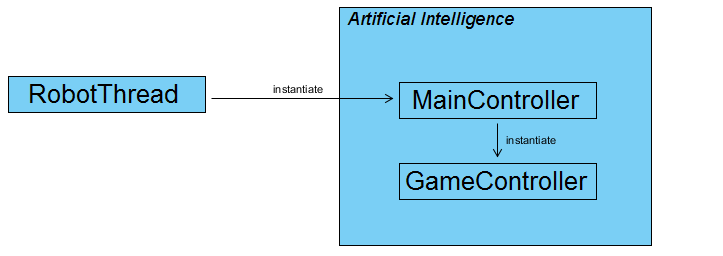
\includegraphics[width=15cm]{images/diagram.png}
\centering
\caption{The MainController thread is started by the robot thread. The MainController then starts the GameController thread.}
\label{thread_diagram}
\end{figure}
\subsection{Description of own classes}
\subsubsection{RobotInteractions}
The RobotInteractions class shown in Figure \ref{class_roboInt} provides methods so that the robot can interact with the game. It contains for example the \emph{close()} and \emph{open()} methods to open and close the gripper of the robot. The method \emph{movePiece(AbstractFame origin, AbstractFrame destination)} can be used to move a game token from one position to another. It uses methods of the RobotMovements class to perform its movements.
\begin{figure}[h]
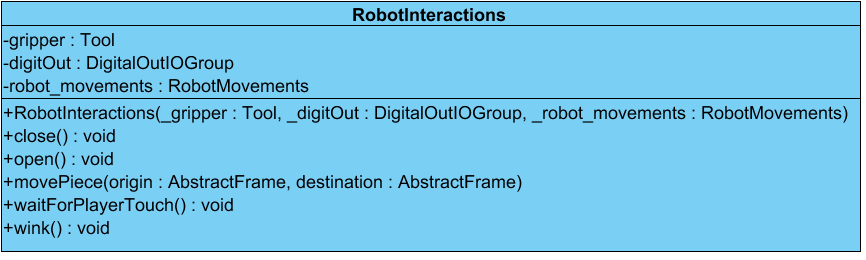
\includegraphics[width=15cm]{images/class_roboInt.png}
\centering
\caption{Class diagram of the RobotInteractions class}
\label{class_roboInt}
\end{figure}

\subsubsection{RobotMovements}
\begin{figure}[h]
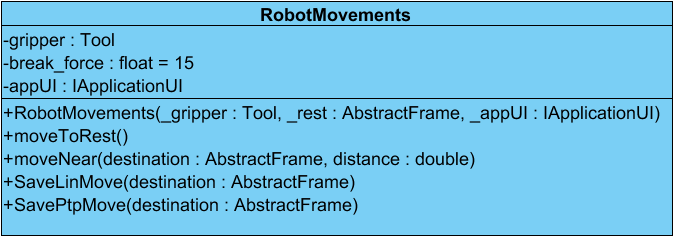
\includegraphics[width=12cm]{images/class_roboMov.png}
\centering
\caption{Class diagram of the RobotMovements class}
\label{class_roboMov}
\end{figure}
The RobotsMovements class shown in Figure \ref{class_roboMov} provides special movement methods like the \emph{moveToRest()} method which moves the robot to its rest position. It also provides the methods \emph{saveLinMove(AbstractFrame destination)} and \emph{savePtpMove(AbstractFrame destination)}. These are methods which where  created to enable safety for the human player. Since the robot is interacting in the same space where the human is also interacting, it is important to ensure that the human player will not be harmed by the robot. \\
\begin{figure}[h]
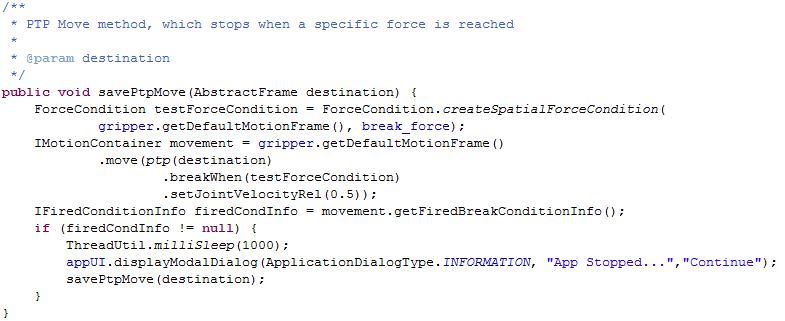
\includegraphics[width=18cm]{images/code_safety.png}
\centering
\caption{Code Listing of the RobotMovements class showing the SavePtpMove() method}
\label{code_safety}
\end{figure}
As shown in Figure \ref{code_safety} the \emph{savePtpMove(AbstractFrame destination)} method calls the \emph{move()} method of the \emph{IMotionContainer} class from the KUKA libraries with a \textit{breakWhen()} condition attached to that. This means that the movement will stop, when the specified ForceCondition will be fired. In case the ForceCondition was fired the movement will be stopped, the robot will wait for a second and a dialog will be shown on the KUKA Smartpad. The user then has to click on this dialog so that the movement can be repeated.
\subsubsection{Bordpoints}
\begin{figure}[h]
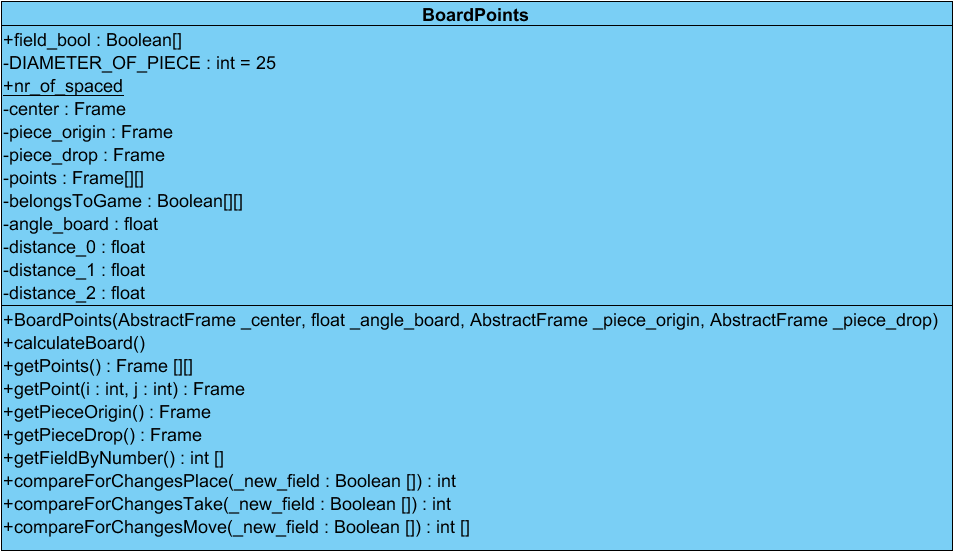
\includegraphics[width=15cm]{images/class_boPo.png}
\centering
\caption{Class diagram of the BoardPoints class}
\label{class_boPo}
\end{figure}
The BoardPoints class shown in Figure \ref{class_boPo} provides  all the information about important coordinates. At the start of the application this class calculates the coordinates for all 24 board points and stores them in a multidimensional array. \\
\begin{figure}[h]
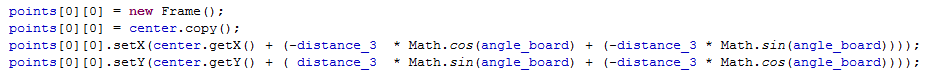
\includegraphics[width=17cm]{images/code_points_calc.png}
\centering
\caption{Code Listing of the Boardpoints class showing the board points calculation}
\label{code_points_calc}
\end{figure}
Figure \ref{code_points_calc} shows the calculation for the board point 0, 0 which is the point in the lower left corner. The calculation uses the center point of the board and the angle of rotation of the board to calculate the coordinates for each game point. The plan was to  get the center point and the angle of the board from the camera, but unfortunately the detection of the created jobs was not precise enough to get the correct angle of the board. So in this project the board needed to stay at a fixed angle. But with a correct working method to get the current angle from e.g. the camera this class is already prepared to compute the points based on the rotation of the board.

\subsubsection{Logger}
\begin{figure}[h]
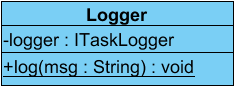
\includegraphics[width=4cm]{images/class_lo.png}
\centering
\caption{Class diagram of the Logger class}
\label{class_lo}
\end{figure}
The logger class shown in Figure \ref{class_lo} is instantiated as a static object in the main thread. This way logging information for debug messages or game messages could be used anywhere in the code.
\subsubsection{ModbusClient}
\begin{figure}[h]
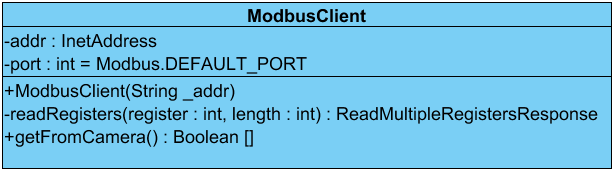
\includegraphics[width=12cm]{images/class_moCli.png}
\centering
\caption{Class diagram of the ModbusClient class}
\label{class_moCli}
\end{figure}
The ModbusClient class shown in Figure \ref{class_moCli} is responsible for the communication between the camera and the robot. As described in section \ref{commu} the communication is realized with Modbus/TCP. The ModbusClient class is instantiated inside the GameController of the artificial intelligence. The GameController calls the \emph{getFromCamera()} method which uses the \emph{readRegisters(int register, int length)} method to read the specified registers from the Modbus/TCP server provided by the camera. 

\subsection{Visual analysis}
The visual analysis of the game was realized with an Cognex In-Sight 7000 Integrated Vision System. 
\subsubsection{In-Sight Explorer}
With the help of the Cognex In-Sight Explorer it was possible to create jobs to analyze the image captured by the camera.\\
\begin{figure}[h]
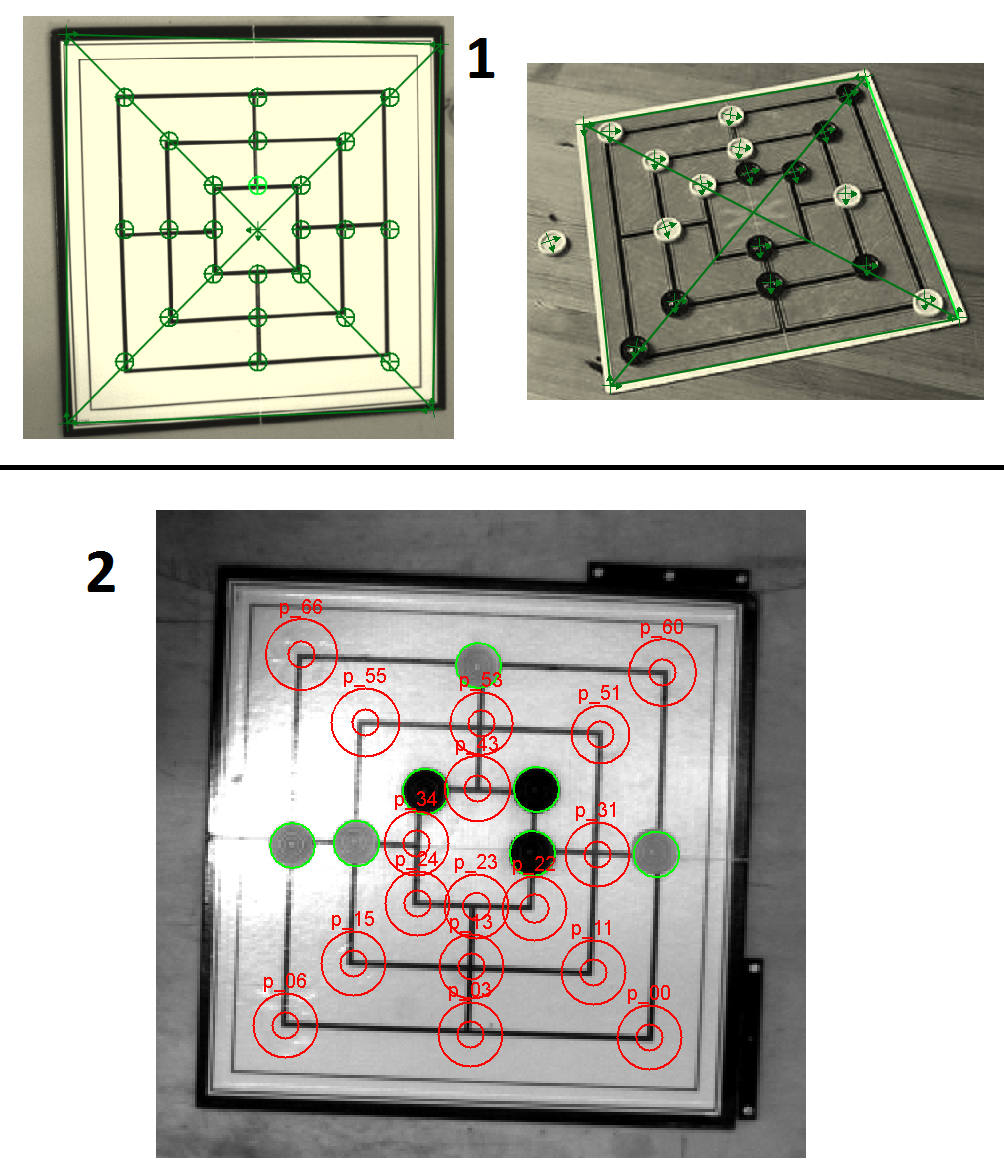
\includegraphics[width=15cm]{images/camera_00.png}
\centering
\caption{Different approaches for visual analysis}
\label{camera_00}
\end{figure}
It was the intention to create a job that can analyze the positions of game tokens on the board considering the rotation of the board. To accomplish this the job should detect the corners of the game board. These corners then could be connected. The intersection between the two lines that cross the game board will be the center of the game board (See Figure \ref{camera_00} part one). Comparing the angle of one of the lines with a reference line with an angle of 0 degrees provides the information about the rotation of the game board.\\ Unfortunately the detection of the board corners did not work as precise as needed. This lead to the problem that the rotation of the board could not be analyzed correctly. A wrong angle of the board would lead to wrong calculations for the board points. Since it is important, that the location of the board points are precise, so that the robot moves and takes pieces from the correct coordinates, the decision was made to use a fixed rotation for the game board. This is a limitation that could be resolved in a following project.\\
The detection of the tokens is realized with a tool of the In-Sight Explorer that detects circles at specific locations. It will output a message "available", if a circle was found at this location and another message "not available", if no circle was found at this location. The tool is not able to determine the color of the found circles. But since nine men's  morris is a game, that is played in turns, we can get the information about the color of the tokens within the robot application. On the downside, this limits the ability of cheat or misplaced game token detection.


\subsubsection{Communication between Robot and Camera}
\label{commu}
The communication as shown in Figure \ref{communication} uses the Modbus/TCP protocol. The camera acts as an Modbus/TCP server and the robot as Modbus/TCP client. The \emph{ModbusClient} class of the robot application (see Figure \ref{class_moCli})  sends a \emph{ReadMultipleRegistersRequest()} to the IP and port of the camera. The camera then sends the output of the visual analysis as TCP packages back to the robot application. The response of the camera is stored as an array of 24 boolean values inside the robot application where \emph{true} means a token was found and \emph{false} means no token was found at this location. This array can now be compared to the previously stored array \emph{field\_bool} in the \emph{BoardPoints} class (see Figure \ref{class_boPo}).
\begin{figure}[h]
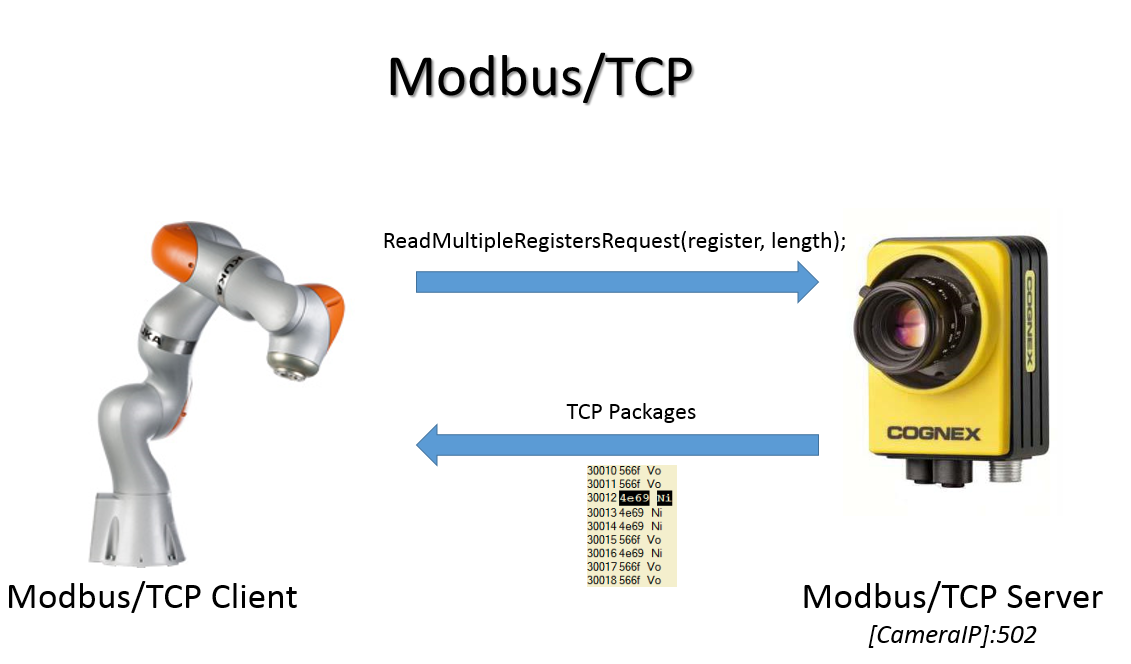
\includegraphics[width=15cm]{images/communication.png}
\centering
\caption{Communication between Camera and Robot}
\label{communication}
\end{figure}


\section{Conclusion and Future work}
\end{large}
\newpage

%%%%%%%%%%%%%%%%%%%%%%%%%%%%%%%%%%%%%%%%%%%%%%%%%%%%%%%%%%%%%
%%%%% References %%%%%
\bibliographystyle{babunsrt-lf}
%\bibliographystyle{spiebib}   %>>>> makes bibtex use spiebib.bst
\bibliography{references}   %>>>> bibliography data in report.bib


\end{document} 
